\documentclass[12pt]{book}

\newcommand{\thetitle}{Think Java: How to Think Like a Computer Scientist}
\title{\thetitle}

\newcommand{\theauthors}{Allen Downey and Chris Mayfield}
\author{\theauthors}

\newcommand{\theversion}{Version 6.0 Draft -- \today}
\date{\theversion}

\usepackage{geometry}
\geometry{
    width=5.5in,
    height=8.5in,
    hmarginratio=3:2,
    vmarginratio=1:1,
    includehead=true,
    headheight=15pt
}

% paragraph spacing
\setlength{\parindent}{0pt}                      % 17.62482pt
\setlength{\parskip}{12pt plus 4pt minus 4pt}    % 0.0pt plus 1.0pt
\linespread{1.05}
\def\arraystretch{1.5}

% list spacing
\setlength{\topsep}{5pt plus 2pt minus 3pt}      % 10.0pt plus 4.0pt minus 6.0pt
\setlength{\partopsep}{-6pt plus 2pt minus 2pt}  %  3.0pt plus 2.0pt minus 2.0pt
\setlength{\itemsep}{0pt}                        %  5.0pt plus 2.5pt minus 1.0pt

% these are copied from tex/latex/base/book.cls
% all I changed is afterskip
\makeatletter
\renewcommand{\section}{\@startsection {section}{1}{\z@}%
    {-3.5ex \@plus -1ex \@minus -.2ex}%
    {0.7ex \@plus.2ex}%
    {\normalfont\Large\bfseries}}
\renewcommand\subsection{\@startsection{subsection}{2}{\z@}%
    {-3.25ex\@plus -1ex \@minus -.2ex}%
    {0.3ex \@plus .2ex}%
    {\normalfont\large\bfseries}}
\renewcommand\subsubsection{\@startsection{subsubsection}{3}{\z@}%
    {-3.25ex\@plus -1ex \@minus -.2ex}%
    {0.3ex \@plus .2ex}%
    {\normalfont\normalsize\bfseries}}
\makeatother

% table of contents vertical spacing
\usepackage{tocloft}
\setlength\cftparskip{8pt plus 4pt minus 4pt}

% The following line adds a little extra space to the column
% in which the Section numbers appear in the table of contents
\makeatletter
\renewcommand{\l@section}{\@dottedtocline{1}{1.5em}{3.0em}}
\makeatother

% customize page headers
\usepackage{fancyhdr}
\pagestyle{fancyplain}
\renewcommand{\chaptermark}[1]{\markboth{Chapter \thechapter ~~ #1}{}}
\renewcommand{\sectionmark}[1]{\markright{\thesection ~~ #1}}
\lhead[\fancyplain{}{\bfseries\thepage}]%
      {\fancyplain{}{\bfseries\rightmark}}
\rhead[\fancyplain{}{\bfseries\leftmark}]%
      {\fancyplain{}{\bfseries\thepage}}
\cfoot{}
%\rfoot{\textcolor{gray}{\tiny ThinkJava Draft \today}}

% balanced index with TOC entry
\usepackage{makeidx}
\makeindex
%\usepackage[totoc]{idxlayout}

% automatically index glossary terms
\newcommand{\term}[1]{%
\index{#1}
\item[#1:]}
% TODO: doesn't work with plastex
%\newcommand{\term}[1]{\item[#1:]}

% where to find graphics
\usepackage{graphicx}
%\graphicspath{{figs/}}

%% tweak spacing of figures and captions
%\usepackage{floatrow}
%\usepackage{caption}
%\captionsetup{
%    font=small,
%    labelformat=empty,
%    justification=centering,
%    skip=4pt
%}

% format end of chapter excercises
\usepackage{amsmath}
\usepackage{amsthm}
\newtheoremstyle{exercise}
  {12pt}        % space above
  {12pt}        % space below
  {}            % body font
  {}            % indent amount
  {\bfseries}   % head font
  {}            % punctuation
  {12pt}        % head space
  {}            % custom head
\theoremstyle{exercise}
\newtheorem{exercise}{Exercise}[chapter]

% colors for code listings and output
\usepackage{xcolor}
\definecolor{bgcolor}{HTML}{FAFAFA}
\definecolor{comment}{HTML}{007C00}
\definecolor{keyword}{HTML}{0000FF}
\definecolor{strings}{HTML}{B20000}

% syntax highlighting in code listings
\usepackage{textcomp}
\usepackage{listings}
\lstset{
    language=java,
    basicstyle=\ttfamily,
    backgroundcolor=\color{bgcolor},
    commentstyle=\color{comment},
    keywordstyle=\color{keyword},
    stringstyle=\color{strings},
    columns=fullflexible,
    keepspaces=true,
    showstringspaces=false,
    upquote=true,
    aboveskip=\parskip,
    belowskip=\parskip
}

% code listing environments
\lstnewenvironment{code}
{\minipage{\linewidth}}
{\endminipage}
\lstnewenvironment{stdout}
{\lstset{commentstyle=,keywordstyle=,stringstyle=}\minipage{\linewidth}}
{\endminipage}

% pdf hyperlinks, table of contents, and document properties
\usepackage[pdftex]{hyperref}
\hypersetup{%
  pdftitle={\thetitle},
  pdfauthor={\theauthors},
  pdfsubject={\theversion},
  pdfkeywords={},
  bookmarksopen=false,
  colorlinks=true,
  citecolor=black,
  filecolor=black,
  linkcolor=black,
  urlcolor=blue
}

% inline syntax formatting
\newcommand{\java}[1]{\lstinline{#1}} %\end{
%\newcommand{\java}[1]{\verb"#1"}
%\newcommand{\java}[1]{{\tt #1}}

\begin{document}
\setcounter{chapter}{11}


\chapter{Arrays of Objects}

In the remaining chapters, we will develop programs that work with playing cards and decks of cards.
Here is an outline of the road ahead:

\begin{enumerate}

\item In this chapter, we will define a \java{Card} class and write methods that work directly with \java{Card}s and arrays of \java{Card}s.

%TODO add \ref for each chapter

\item In Chapter 13, we will create a \java{Deck} class that encapsulates an array of Cards and write methods that operate on \java{Deck}s.

\item In Chapter 14, we will introduce object-oriented programming (OOP) and redesign the \java{Card} and \java{Deck} classes accordingly.

\end{enumerate}

Although we will see several versions of the same code, the main advantage of proceeding this way is that the explanations will be smoother.
It may help you to create a {\tt Card.java} file and paste in the examples as we go.

%If it helps, you can download the code for each chapter as you go along.
%The code for this chapter is here: \url{http://thinkapjava.com/code/Card1.java}.


\section{Card objects}
\label{card}

\index{Card}
\index{class!Card}

If you are unfamiliar with traditional playing cards, now would be a good time to get a deck; otherwise this chapter might not make much sense.
Or just read \url{https://en.wikipedia.org/wiki/Standard_52-card_deck}.

\index{rank}
\index{suit}

There are 52 cards in a standard deck.
Each card belongs to one of four suits and one of 13 ranks.
The suits are Spades, Hearts, Diamonds, and Clubs (in descending order in Bridge).
The ranks are Ace, 2, 3, 4, 5, 6, 7, 8, 9, 10, Jack, Queen, and King.
Depending on what game you are playing, the Ace may be considered higher than King or lower than 2.

If we want to define a new object to represent a playing card, it is pretty obvious what the instance variables should be: \java{rank} and \java{suit}.
It is not as obvious what types the instance variables should be.
One possibility is \java{String}s, containing things like \java{"Spade"} for suits and \java{"Queen"} for ranks.
A problem with this implementation is that it would not be easy to compare cards to see which had higher rank or suit.

\index{encode}
\index{encrypt}
\index{map to}

An alternative is to use integers to {\bf encode} the ranks and suits.
By ``encode'' we do not mean to encrypt or translate into a secret code.
What a computer scientist means by encode is something like ``define a mapping between a sequence of numbers and the things we want to represent.''

\begin{tabular}{l c l}
Clubs & $\mapsto$ & 0 \\
Diamonds & $\mapsto$ & 1 \\
Hearts & $\mapsto$ & 2 \\
Spades & $\mapsto$ & 3
\end{tabular}

The nice feature of this mapping is that the suits map to integers in order, so we can compare suits simply by comparing integers.
The mapping for ranks is fairly obvious: each of the numerical ranks maps to the corresponding integer, and for face cards:

\begin{tabular}{l c l}
Ace & $\mapsto$ & 1 \\
Jack & $\mapsto$ & 11 \\
Queen & $\mapsto$ & 12 \\
King & $\mapsto$ & 13 \\
\end{tabular}

The reason we are using mathematical notation for these mappings is that they are not part of the program.
They are part of the program design, but they never appear explicitly in the code.
The class definition for the \java{Card} type simply looks like this:

\begin{code}
public class Card {
    private int suit;
    private int rank;

    public Card() {
        this.suit = 0;
        this.rank = 0;
    }

    public Card(int suit, int rank) {
        this.suit = suit;
        this.rank = rank;
    }
}
\end{code}

\index{constructor}

As usual, we define two constructors: a default constructor that takes no parameters, and an explicit value constructor that takes a parameter for each instance variable.
To create a \java{Card} object that represents the 3 of Clubs, we can invoke the \java{new} operator:

\begin{code}
    Card threeOfClubs = new Card(0, 3);
\end{code}

%The first argument, \java{0} represents the suit Clubs.


\section{The printCard method}
\label{printcard}

\index{print!Card}

When you create a new class, the first step is to declare the instance variables and write constructors.
The second step is to write the standard methods that every object should have, including one that prints the object, and one or two that compare objects.
Let's start with \java{printCard}.

\index{String!array of}
\index{array!of String}

To print \java{Card} objects in a way that humans can read easily, we need to map the integer codes onto words.
A natural way to do that is with an array of \java{String}s.
You can create an array of \java{String}s the same way you create an array of primitive types:

\begin{code}
    String[] suits = new String[4];
\end{code}

Then we can set the values of the elements of the array.

\begin{code}
    suits[0] = "Clubs";
    suits[1] = "Diamonds";
    suits[2] = "Hearts";
    suits[3] = "Spades";
\end{code}

Creating an array and initializing the elements is such a common operation that Java provides a special syntax for it:

\begin{code}
    String[] suits = {"Clubs", "Diamonds", "Hearts", "Spades"};
\end{code}

\index{memory diagram}

This statement is equivalent to the separate declaration, allocation, and assignment.
The memory diagram of this array looks like:

\begin{center}
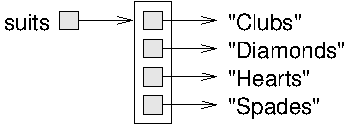
\includegraphics{figs/stringarray.pdf}
\end{center}

\index{reference}
\index{String!reference to}

Notice how the elements of the array are {\em references} to the \java{String}s, rather than \java{String}s themselves.

Now we need another array of \java{String}s to decode the ranks:

\begin{code}
    String[] ranks = {"narf", "Ace", "2", "3", "4", "5", "6",
               "7", "8", "9", "10", "Jack", "Queen", "King"};
\end{code}

The reason for the \java{"narf"} is to act as a place-keeper for thezeroeth element of the array, which is never used (or shouldn't be).
The only valid ranks are 1--13.
To avoid this wasted element, we could have started at 0, but the mapping is more natural if we encode 2 as 2, 3 as 3, and so forth.

Using these arrays, we can select the appropriate \java{String}s by using the \java{suit} and \java{rank} as indexes.
In the method \java{printCard}:

\begin{code}
public static void printCard(Card c) {
    String[] suits = {"Clubs", "Diamonds", "Hearts", "Spades"};
    String[] ranks = {"narf", "Ace", "2", "3", "4", "5", "6",
               "7", "8", "9", "10", "Jack", "Queen", "King"};
    System.out.println(ranks[c.rank] + " of " + suits[c.suit]);
}
\end{code}

The expression \java{suits[c.suit]} means ``use the instance variable \java{suit} from the object \java{c} as an index into the array named \java{suits}.''

\begin{code}
    Card card = new Card(1, 11);
    printCard(card);
\end{code}

The output for this code is {\tt Jack of Diamonds}.


\section{The sameCard method}
\label{equivalence}

The word ``same'' is one of those things that occur in natural language that seem perfectly clear until you give it some thought, and then you realize there is more to it than you expected.

\index{natural language}
\index{language!natural}

For example, if I say ``Jared and I have the same car,'' I mean that his car and mine are the same make and model, but they are
two different cars.
If I say ``Jared and I have the same mother,'' I mean that his mother and mine are one person.
So the idea of ``sameness'' is different, depending on the context.

\index{ambiguity}

When you talk about objects, there is a similar ambiguity.
For example, if two \java{Card}s are the same, does that mean they contain the same data (rank and suit), or they are actually
the same \java{Card} object?

\index{identical}

To see if two references refer to the same object, we use the \java{==} operator.
References to the same object are {\bf identical}.
For example:

\begin{code}
    Card card1 = new Card(1, 11);
    Card card2 = card1;

    if (card1 == card2) {
        System.out.println("card1 and card2 are identical");
    }
\end{code}

\index{equivalent}

In contrast, references to objects with same data are {\bf equivalent}.
To check equivalence, it is common to write a method with a name like \java{sameCard}.

\begin{code}
    public static boolean sameCard(Card c1, Card c2) {
        return c1.suit == c2.suit && c1.rank == c2.rank;
    }
\end{code}

Here is an example that creates two objects with the same data, and uses \java{sameCard} to see if they are equivalent:

\begin{code}
    Card card1 = new Card(1, 11);
    Card card2 = new Card(1, 11);

    if (sameCard(card1, card2)) {
        System.out.println("card1 and card2 are equivalent");
    }
\end{code}

Note that if references are identical, they are also equivalent.
However if they are equivalent, they are not necessarily identical.
In the above example, \java{card1} and \java{card2} are equivalent but not identical.
Here is a memory diagram:

\begin{center}
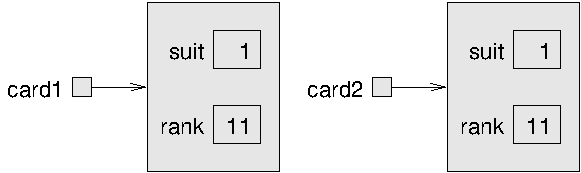
\includegraphics{figs/card.pdf}
\end{center}

%\index{aliasing}
%What does it look like when \java{card1} and \java{card2} are identical?

%In Section~\ref{incomparable} I said that you should not use the \java{==} operator on \java{String}s because it does not do what you expect.
%Instead of comparing the contents of the \java{String} (equivalence), it checks whether the two \java{String}s are the same object (identity).


\section{The compareCard method}
\label{compare}

\index{compareCard}
\index{operator!conditional}
\index{conditional operator}

For primitive types, the conditional operators compare values and determine when one is greater or less than another.
These operators (\java{<}, \java{>}, and others) don't work for object types.
For \java{String}s, Java provides a \java{compareTo} method.
We have to write our own version for \java{Card}s, which we will call \java{compareCard}.
Later we will use this method to sort a deck of cards.

\index{ordering}
\index{complete ordering}
\index{partial ordering}

Some types are completely ordered, which means that you can compare any two values and tell which is bigger.
Integers and floating-point numbers are totally ordered.
Some sets are unordered, which means that there is no meaningful way to say that one element is bigger than another.
Fruits are unordered, which is why we cannot compare apples and oranges.
In Java, the \java{boolean} type is unordered; we cannot say that \java{true} is greater than \java{false}.

The set of playing cards is partially ordered, which means that sometimes we can compare cards and sometimes not.
For example, I know that the 3 of Clubs is higher than the 2 of Clubs, and the 3 of Diamonds is higher than the 3 of Clubs.
But which is better, the 3 of Clubs or the 2 of Diamonds?
One has a higher rank, but the other has a higher suit.

\index{comparable}

To make cards comparable, we have to decide which is more important: rank or suit.
The choice is arbitrary, but when you buy a new deck of cards, it comes sorted with all the Clubs together, followed by all the Diamonds, and so on.
So for now, let's say that suit is more important.

With that decided, we can write \java{compareCard}.
It takes two \java{Card}s as parameters and returns 1 if the first card wins, -1 if the second card wins, and 0 if they are equivalent.
First we compare suits:

\begin{code}
    if (c1.suit > c2.suit) {
        return 1;
    }
    if (c1.suit < c2.suit) {
        return -1;
    }
\end{code}

If neither statement is true, then the suits must be equal and we have to compare ranks:

\begin{code}
    if (c1.rank > c2.rank) {
        return 1;
    }
    if (c1.rank < c2.rank) {
        return -1;
    }
\end{code}

If neither of these is true, then the ranks must also be equal.
So we simply return 0 at the end of the method.


\section{Class variables}

So far we have seen local variables, which are declared inside a method, and instance variables, which are declared in a class
definition, usually before the method definitions.
Local variables are created when a method is invoked and destroyed when the method ends.
Instance variables are created when you create an object and destroyed when the object is garbage collected.

\index{class variables}

Now it's time to learn about {\bf class variables}.
Like instance variables, class variables are defined in a class definition before the method definitions.
But they are identified by the keyword \java{static}.
They are created when the program starts (or when the class is used for the first time) and survive until the program ends.
Class variables are {\em shared} across all instances of the class.

You can refer to a class variable from anywhere inside the class definition.
Class variables are often used to store constant values that are needed in several places.
In that case, they should also be defined as \java{final}.
Note that whether a variable is \java{static} or \java{final} involves two separate considerations:
\java{static} means the variable is shared, and \java{final} means the variable is constant.

As an example, here is a version of \java{Card} where \java{suits} and \java{ranks} are defined as class constants:

\begin{code}
public class Card {

    public static final String[] SUITS = {
        "Clubs", "Diamonds", "Hearts", "Spades"};

    public static final String[] RANKS = {
        "narf", "Ace", "2", "3", "4", "5", "6", "7", "8", "9",
        "10", "Jack", "Queen", "King"};

    // instance variables and constructors go here

    public static void printCard(Card c) {
        String name = RANKS[c.rank] + " of " + SUITS[c.suit];
        System.out.println(name);
    }
}
\end{code}

Inside \java{printCard} we can refer to \java{SUITS} and \java{RANKS} as if they were local variables.
Writing \java{static final} variables in ALL CAPS is a common convention that makes it easier to recognize their purpose in the class.

One advantage of defining \java{SUITS} and \java{RANKS} as class variables is that they don't need to be created (and garbage collected) every time the printCard method is called.
They may also be useful in other methods and classes, so it's nice to maintain them in one place.


\section{Arrays of cards}
\label{cardarray}

\index{array!of object}
\index{object!array of}
\index{deck}

\index{composition}

By now we have seen several examples of composition (the ability to combine language features in a variety of arrangements).
One of the first examples we saw was using a method invocation as part of an expression.
Another example is the nested structure of statements: you can put an \java{if} statement within a \java{while} loop, or within
another \java{if} statement, etc.

Having seen this pattern, and having learned about arrays and objects, you should not be surprised to learn that you can make arrays of objects.
And you can define objects with arrays as instance variables; you can make arrays that contain arrays; you can define objects that contain objects, and so on.
%In the next two chapters we will see examples of these combinations using \java{Card} objects.
This example creates an array of 52 cards:

\begin{code}
    Card[] cards = new Card[52];
\end{code}

\index{state diagram}

Here is the memory diagram for this object:

\begin{center}
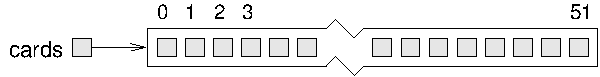
\includegraphics{figs/cardarray.pdf}
\end{center}

\index{null}

The array contains {\em references} to objects; it does not contain the \java{Card} objects themselves.
The elements are initialized to \java{null}.
You can access the elements of the array in the usual way:

\begin{code}
    if (cards[0] == null) {
        System.out.println("No card yet!");
    }
\end{code}

\index{exception!NullPointer}
\index{run-time error}

But if you try to access the instance variables of the non-existent \java{Card}s, you will get a \java{NullPointerException}.

\begin{code}
    System.out.println(cards[0].rank);  // NullPointerException
\end{code}

\index{composition}

That {\em is} the correct syntax for accessing the \java{rank} of the ``zeroeth'' card in the deck.
It's also another example of composition, or combining the syntax for accessing an element of an array and an instance variable of an object.

\index{loop!nested}

The easiest way to populate the deck with \java{Card} objects is to write nested for loops (i.e., one loop inside the body of another):

\begin{code}
    int index = 0;
    for (int suit = 0; suit <= 3; suit++) {
        for (int rank = 1; rank <= 13; rank++) {
            cards[index] = new Card(suit, rank);
            index++;
        }
    }
\end{code}

The outer loop enumerates the suits from 0 to 3.
For each suit, the inner loop enumerates the ranks from 1 to 13.
Since the outer loop runs 4 times, and the inner loop runs 13 times, the body is executed is 52 times.

\index{index}

We use a separate variable \java{index} to keep track of where in the deck the next card should go.
The following memory diagram shows what the deck looks like after the first two cards have been allocated:

\begin{center}
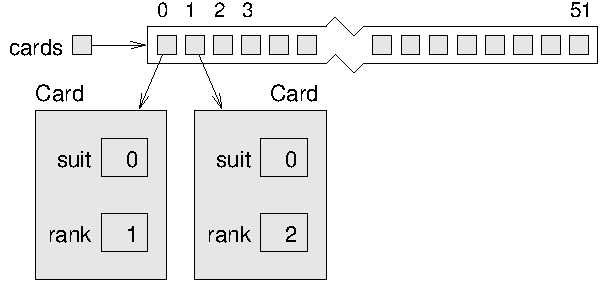
\includegraphics{figs/cardarray2.pdf}
\end{center}


%\section{The printDeck method}
%\label{printdeck}

\index{printDeck}
\index{print!array of Cards}

When you work with arrays, it is convenient to have a method that prints the contents.
We have seen the pattern for traversing an array several times, so the following method should be familiar:

\begin{code}
    public static void printDeck(Card[] cards) {
        for (int i = 0; i < cards.length; i++) {
            printCard(cards[i]);
        }
    }
\end{code}

Since \java{cards} has type \java{Card[]}, an element of \java{cards} has type \java{Card}.
So \java{cards[i]} is a legal argument for \java{printCard}.


\section{Sequential search}
\label{findcard}

\index{findCard}
\index{sequential search}
\index{binary search}

The next method we'll write is \java{findCard}, which searches an array of \java{Card}s to see whether it contains a certain card.
This method gives us a chance to demonstrate two algorithms: {\bf sequential search} and {\bf binary search}.

\index{traverse}
\index{loop!search}

Sequential search is pretty obvious: we traverse the deck and compare each card to the one we are looking for.
If we find it, we return the index where the card appears.
If it is not in the deck, we return -1.

\begin{code}
public static int findCard(Card[] cards, Card card) {
    for (int i = 0; i< cards.length; i++) {
        if (sameCard(cards[i], card)) {
            return i;
        }
    }
    return -1;
}
\end{code}

The parameters of \java{findCard} are \java{cards} and \java{card}.
It might seem odd to have a variable with the same name as a type (the \java{card} variable has type \java{Card}).
We can tell the difference because the variable begins with a lower-case letter.

\index{statement!return}
\index{return!inside loop}

The method returns as soon as it discovers the card, which means that we do not have to traverse the entire deck if we find the card we are looking for.
If we get to the end of the loop, however, we know the card is not in the deck.

If the cards in the deck are not in order, there is no way to search faster than sequential search.
We have to look at every card, because otherwise we can't be certain the card we want is not there.

However for large arrays, sequential search is rather inefficient.
If you pay the price to keep them sorted, finding elements becomes much easier.


\section{Binary search}

When you look for a word in a dictionary, you don't just search page by page from front to back.
Since the words are in alphabetical order, you probably use an algorithm similar to binary search:

\begin{enumerate}
\item Start in the middle of the dictionary (or array).
\item Compare a word on that page to the word you are looking for.
If you find the word you are looking for, stop.
\item If the word you are looking for comes after the word on the page, flip to somewhere later in the dictionary and go back to step 2.
\item If the word you are looking for comes before the word on the page, flip to somewhere earlier in the dictionary and go back to step 2.
\end {enumerate}

If you ever get to the point where there are two adjacent words on the page and your word comes between them, you can conclude that your word is not in the dictionary.

Getting back to the deck of cards, we can write a faster version of \java{findCard} if we know the cards are in order.
It takes a little more code, but the idea is the same four steps listed above.

\begin{code}
public static int findCard(Card[] cards, Card card) {
    int low = 0;
    int high = cards.length - 1;
    while (low <= high) {
        int mid = (low + high) / 2;                   // step 1
        int comp = compareCard(cards[mid], card);

        if (comp == 0) {                              // step 2
            return mid;
        } else if (comp < 0) {                        // step 3
            low = mid + 1;
        } else {                                      // step 4
            high = mid - 1;
        }
    }
    return -1;
}
\end{code}

First, we declare \java{low} and \java{high} variables to represent the range we are searching.
Initially we search the entire array, from index \java{0} to \java{length - 1}.
We will terminate our search if these indexes ever cross, yielding an invalid range.

Inside the \java{while} loop, we repeat the four steps of binary search:

\begin{enumerate}

\item To search the array, choose an index between \java{low} and \java{high} (call it \java{mid}) and compare it to the card you are looking for.

\item If you found it, return the index.

\item If the card at \java{mid} is higher than your card, search the range from \java{low} to \java{mid - 1}.

\item If the card at \java{mid} is lower than your card, search the range from \java{mid + 1} to \java{high}.

\end{enumerate}

%\section{Recursive version}

\index{recursion}

Another way to write a binary search is with a recursive method.
The trick is to write a method that takes \java{low} and \java{high} as parameters, and turn steps 3 and 4 into recursive invocations.
%They indicate the segment of the array that should be searched (including both \java{low} and \java{high}).
Here's what this algorithm looks like translated into Java code:

\begin{code}
public static int findCard(Card[] cards, Card card,
                           int low, int high) {
    if (high < low) {
        return -1;
    }
    int mid = (low + high) / 2;                       // step 1
    int comp = compareCard(cards[mid], card);

    if (comp == 0) {                                  // step 2
        return mid;
    } else if (comp < 0) {                            // step 3
        return findCard(cards, card, mid + 1, high);
    } else {                                          // step 4
        return findCard(cards, card, low, mid - 1);
    }
}
\end{code}

%This code contains the main idea of a binary search, but it is still missing an important part.
%As written, the method recurses forever if the card is not in the deck!
%We need a base case to handle this condition and end the recursion.

Instead of a \java{while} loop, we simply have an \java{if} statement to terminate the recursion.
If \java{high} is less than \java{low}, there are no cards between them, and we conclude that the card is not in the deck.
%We can handle that case by adding a single \java{if} statement to the top:

\index{recursion!infinite}
\index{infinite recursion}
\index{exception!StackOverflow}

Two common errors in recursive programs are (1) forgetting to include a base case, and (2) writing the recursive call so that the base case is never reached.
Either error causes infinite recursion and a \java{StackOverflowException}.
%(Think of a stack diagram for a recursive method that never ends.)

\section{Tracing the code}

To see how binary search works, it's useful to add the following print statement at the beginning of each iteration (or recursive call).

\begin{code}
    System.out.println(low + ", " + high);
\end{code}

%The print statement is unnecessary, but it's useful to trace the sequence of recursive invocations.

Then in the \java{main} method, execute the following code (after creating the cards array with nested loops):

\begin{code}
    Card card = new Card(1, 11);
    System.out.println(findCard(cards, card));
\end{code}

The result is \java{23} as expected, since there are 13 cards in the zeroth suit followed by 11 in the first suit (and indexes start at zero).
Here is the complete output, thanks to the print statement in \java{findCard}:

\begin{stdout}
0, 51
0, 24
13, 24
19, 24
22, 24
23
\end{stdout}

Let's make up a card that is not in the deck, say \java{new Card(1, 15)} or the ``15 of Diamonds''.
If we try to find it using binary search, we get the following:

\begin{stdout}
0, 51
26, 51
26, 37
26, 30
26, 27
26, 25
-1
\end{stdout}

%\index{testing}
%\index{correctness}
%
%These tests don't prove that this program is correct.
%In fact, no amount of testing can {\em prove} that a program is correct.
%But looking at a few cases and examining the code, you might be able to convince yourself.

Binary search over an array of length $n$ requires $\log_2 n$ comparisons.
So we only have to look at 5 or 6 cards in the deck, as opposed to all 52 if we did a sequential search.
In general, binary search is much faster than sequential search (which requires $n$ comparisons), and even more so for large arrays.


\section{Vocabulary}

\begin{description}

\term{encode}
To represent one set of values using another set of values, by constructing a mapping between them.

\term{identical}
Equality of references.
Two references that point to the same object in memory.

\term{equivalent}
Equality of values.
Two references that point to objects that contain the same data.

\term{class variable}
A variable declared within a class as \java{static}.
There is always exactly one copy of this variable, no matter how many objects exist.

\term{sequential search}
An algorithm that searches array elements in order, one by one, until an item is found.

\term{binary search}
An algorithm that searches an ordered array by starting in the middle and discarding half of the remaining elements each time a comparison is made.

\end{description}


\section{Exercises}


\begin{exercise}
Encapsulate the code in Section~\ref{compare} in a method.
Then modify it so that aces are ranked higher than Kings.
\end{exercise}


\begin{exercise}
Encapsulate the deck-building code from Section~\ref{cardarray} in a method called \java{makeDeck} that takes no parameters and returns a fully-populated array of \java{Card}s.
\end{exercise}


\begin{exercise}
In Blackjack the object of the game is to get a collection of cards with a score of 21.
The score for a hand is the sum of scores for all cards.
The score for an aces is 1, for all face cards is ten, and for all other cards the score is the same as the rank.
For example, the hand (Ace, 10, Jack, 3) has a total score of 1 + 10 + 10 + 3 = 24.

Write a method called \java{handScore} that takes an array of cards as an argument and that returns the total score.
\end{exercise}


\begin{exercise}
In Poker a ``flush'' is a hand that contains five or more cards of the same suit.
A hand can contain any number of cards.

\begin{enumerate}

\item Write a method called \java{suitHist} that takes an array of Cards as a parameter and that returns a histogram of the suits in the hand.
Your solution should only traverse the array once.

\item Write a method called \java{hasFlush} that takes an array of Cards as a parameter and returns \java{true} if the hand contains a flush (\java{false} otherwise).

\end{enumerate}

\end{exercise}


\end{document}
